\section{Klassifizierung}
Statt die genaue Regenmenge vorherzusagen, stellten wir drei Kategorien auf: kein Regen ($= 0mm$), wenig Regen ($\leq 8mm$) und viel Regen ($> 8mm$). Diese Kategorien haben wir als One-Hot-Vector kodiert. `[1, 0, 0]` entspricht hierbei kein Regen, sodass man aus der ersten Dimension der Vorhersage einfach ein Vorschaubild generieren kann aus dem man gleich feststellen kann, ob es am jeweiligen Pixel regnet oder nicht.

Für das Training mit Kategorien kann man nicht mehr den MSE verwenden, hier würde selbst nach 80 Epochen nur "kein Regen" vorhergesagt. Stattdessen wurde als Loss-Funktion die \enquote{Categorical Crossentropy} von Keras verwendet; die binäre Crossentropy können wir nicht verwenden, weil wir mehr als zwei Kategorien verwenden. Die \enquote{Categorical Crossentropy} funktioniert relativ gut, aber es wird ein Blob vorhersagt, der etwas über den Bereich ragt, in dem es eigentlich regnet.

Danach wurde noch die Aktivierungsfunktion für den Output-Layer Sigmoid durch Softmax ersetzt. Dadurch erscheint das Vorschaubild etwas verwaschener, aber der Blob um das Regengebiet wird kleiner und die Differenz zum Referenzbild wird kleiner.

Wenn man die Aktivierungsfunktion der Hidden-Layer (von ReLu) zu Tanh verändert, verbessert sich auch die Kategorisierung: der Blob nähert sich weiter dem Regengebiet aus dem zu vorhersagendem Bild an, ist aber immer noch merkbar größer und franst an den kanten aus.

Als nächstes wird die Metrik "categorical\_accuracy" verwendet, um die Vorhersage zu überwachen. Dadurch kann der Fortschritt beim Trainieren besser überwacht werden.


\subsection{Training}
Für das Training wurden alle Daten der 18 Jahre verwendet, partitioniert in Trainings- und Evaluationsdaten. Als Lossfunktion wurde der MSE verwendet, der den Unterschied über alle Pixel kumuliert (deswegen die hohen Werte in den Abbildungen). Da das Training auf der GPU weniger al 10~Sekunden pro Epoche dauert, wurden gleich 3072 Epochen trainiert.

In Abbildung~\ref{fig:lernkurven} sind die Lernkurven des Trainings nebeneinander dargestellt, links steht das Training des Netzes mit Softmax als Aktivierungsfunktion des Hidden Layer und rechts ist das selbe Netz mit TanH als Aktivierungsfunktion. Man sieht jedoch, dass es ab etwa 1500~Epochen (x-Achse) keine Verbesserungen mehr gibt.

\begin{figure}[ht]
\centering
\begin{subfigure}{0.5\textwidth}
\centering
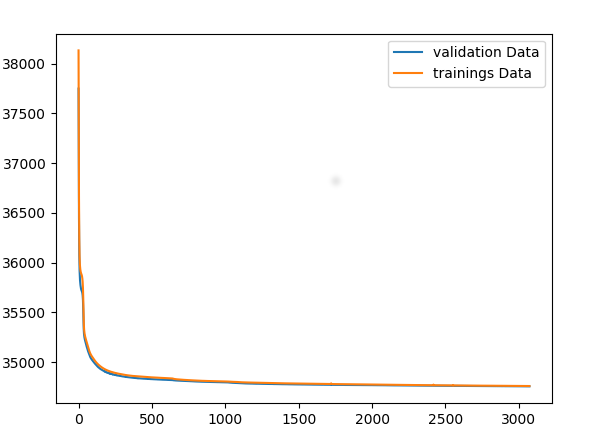
\includegraphics[width=\linewidth]{pics/lernkurve_activationHidden-softmax_activationOutput-softmax}
\caption{Lernkurve (Hidden layer: Softmax)}
\label{fig:lernkurveSoftmax}
\end{subfigure}%
\begin{subfigure}{0.5\textwidth}
\centering
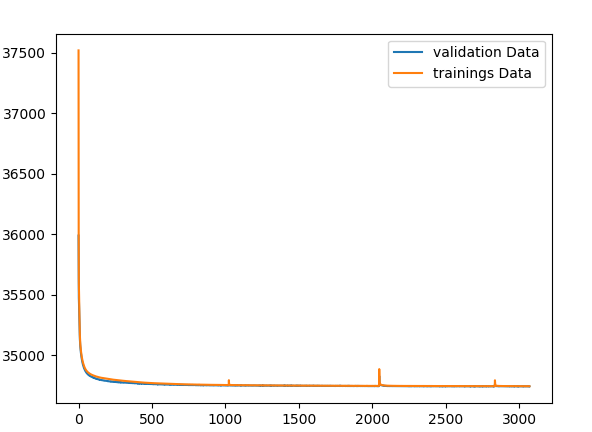
\includegraphics[width=\linewidth]{pics/lernkurve_activationHidden-tanh_activationOutput-softmax}
\caption{Lernkurve (Hidden layer: Tanh)}
\label{fig:lernkurveTanh}
\end{subfigure}%
\caption{Lernkurven von den Aktivierungsfunktionen der Hidden-Layer}
\label{fig:lernkurven}
\end{figure}



\subsection{Auswertung}
Zu den beiden 
In den Confustion-Ma
\begin{table}[ht]
\begin{tabular}{lr|rrr}
                                     &                      & \multicolumn{3}{c}{Vorhersage}\\
                                     &                      & \textbf{Kein Regen}    & \textbf{Wenig Regen}    & \textbf{Viel Regen}\\\hline
\multirow{3}{*}{\rotatebox{90}{Echt}}& \textbf{Kein Regen}  & 2225229                & 35527                   & 3634\\
                                     & \textbf{Wenig Regen} & 76988                  & 110399                  & 17240\\
                                     & \textbf{Viel Regen}  & 8849                   & 27969                   & 45973\\
\end{tabular}
\caption{Confustion-Matrix (Aktivierungsfunktion Hidden Layer: Tanh)}
\label{tab:confusionTanh}
\end{table}

\begin{table}[ht]
\begin{tabular}{lr|rrr}
                                     &                      & \multicolumn{3}{c}{Vorhersage}\\
                                     &                      & \textbf{Kein Regen}    & \textbf{Wenig Regen}    & \textbf{Viel Regen}\\\hline
\multirow{3}{*}{\rotatebox{90}{Echt}}& \textbf{Kein Regen}  & 2227245                & 33383                   & 3762\\
                                     & \textbf{Wenig Regen} & 81116                  & 106434                  & 17077\\
                                     & \textbf{Viel Regen}  & 9695                   & 27930                   & 45166\\
\end{tabular}
\caption{Confustion-Matrix (Aktivierungsfunktion Hidden Layer: Softmax)}
\label{tab:confusionSoftmax}
\end{table}


\begin{figure}[ht]
\centering
\begin{subfigure}{0.5\textwidth}
\centering
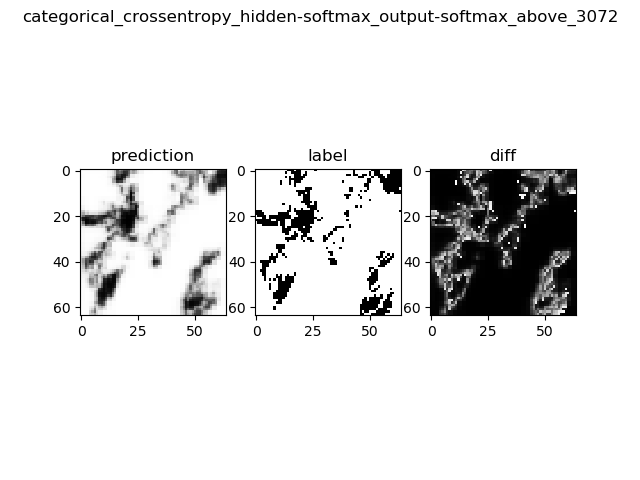
\includegraphics[width=\linewidth]{pics/categorical_crossentropy_hidden-softmax_output-softmax_above_3072}
\caption{Hidden layer activation: Softmax}
\label{fig:hiddenActivationSoftmax}
\end{subfigure}%
\begin{subfigure}{0.5\textwidth}
\centering
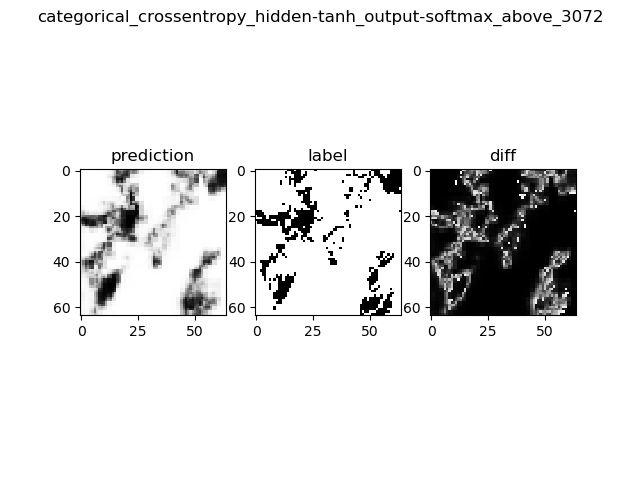
\includegraphics[width=\linewidth]{pics/categorical_crossentropy_hidden-tanh_output-softmax_above_3072}
\caption{Hidden layer activation: Tanh}
\label{fig:hiddenActivationTanh}
\end{subfigure}%
\caption{Vergleich von Aktivierungsfunktionen der Hidden-Layer}
\label{fig:activatinHidden}
\end{figure}


\subsection{Herausforderungen in diesem Kapitel}
\begin{itemize}
\item Richtige Kategorien finden
\item Training mit richtiger Aktivierungsfunktion / Optimizer
\end{itemize}
